Describe and implement a fourth-order Runge-Kutta and Fourier method for the Burger equation with
periodic boundary conditions:

$$u_t = \epsilon u_{xx} + uu_x,\;\;x\in(-\pi,\pi),\;\;u(x,0) = e^{-10\sin^2(x/2)}$$

with $\epsilon = 0.03$ and the simulation running up to $t = 1$.

\begin{solution}\renewcommand{\qedsymbol}{}\ \\
    In order to numerically solve the given PDE, we first initialize our $x$ domain, $\epsilon$, and
    our initial condition. After that, we define some parameters as well as an anonomus function of the
    Fourier transfrom of Burgers equation. Then, we start a loop to implement the Runge-Kutta order
    four method. Then, we sum all of the pieces including the FFT of the initial condition. While still
    in the Runge-Kutta loop, we take this sum and then do the inverse FFT to get back into real space
    and save these values in a matrix. After computing all of these values and saving them to the
    matrix, we plot these values using the waterfall function. AS such, we get the following plot.\\

    \begin{center}
        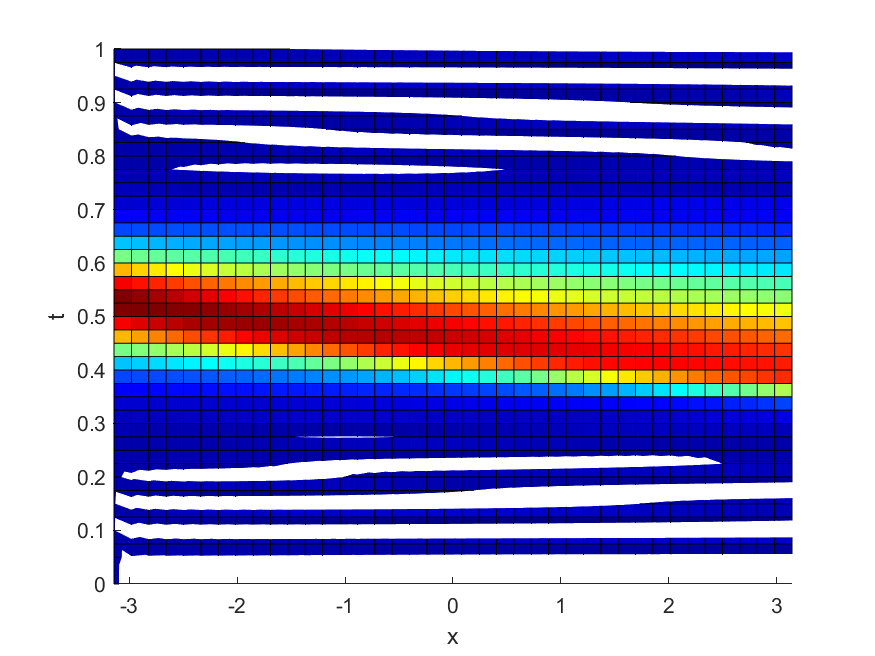
\includegraphics[scale=0.6]{problem1.PNG}
    \end{center}

\end{solution}

\newpage
\lstinputlisting{problem1.m}
\newpage